\documentclass[border=5pt]{standalone}
\usepackage{tikz}
\usetikzlibrary{patterns, arrows.meta, positioning, calc}

\begin{document}
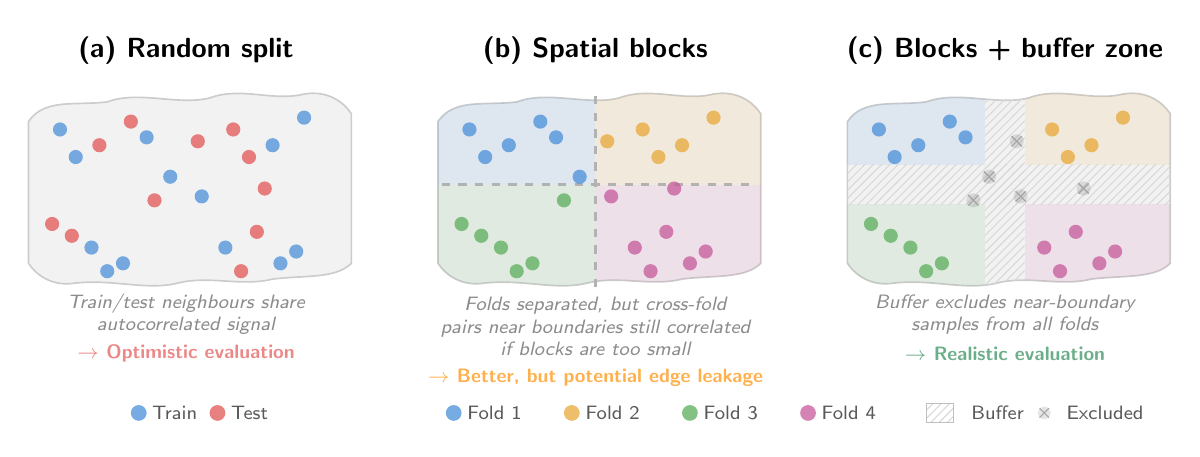
\begin{tikzpicture}[
    >=Stealth,
    every node/.style={font=\sffamily},
    heading/.style={font=\sffamily\normalsize\bfseries},
    sub/.style={font=\sffamily\scriptsize\itshape, text opacity=0.45, align=center},
    annot/.style={font=\sffamily\scriptsize, text opacity=0.7},
    legendlabel/.style={font=\sffamily\scriptsize, text opacity=0.65, anchor=west},
]

% Colors
\definecolor{trainblue}{RGB}{74,144,217}
\definecolor{testred}{RGB}{226,85,85}
\definecolor{foldA}{RGB}{74,144,217}
\definecolor{foldB}{RGB}{232,168,56}
\definecolor{foldC}{RGB}{91,174,91}
\definecolor{foldD}{RGB}{199,90,155}
\definecolor{goodgreen}{RGB}{46,139,87}
\definecolor{midorange}{RGB}{255, 143, 0}

% Dot radius
\def\R{0.09}

% ============================================================
% LAND SHAPE — organic coastline, reused for each panel
% Coordinates in a 4.2 x 3.0 box, origin at bottom-left
% ============================================================
\newcommand{\landpath}{
    (0.1, 2.3) .. controls (0.3, 2.6) and (0.7, 2.5) ..
    (1.1, 2.55) .. controls (1.5, 2.7) and (2.0, 2.5) ..
    (2.4, 2.6) .. controls (2.8, 2.75) and (3.2, 2.55) ..
    (3.6, 2.65) .. controls (3.9, 2.7) and (4.1, 2.55) ..
    (4.2, 2.4)
    -- (4.2, 0.5)
    .. controls (4.0, 0.3) and (3.6, 0.35) ..
    (3.2, 0.3) .. controls (2.8, 0.2) and (2.4, 0.35) ..
    (2.0, 0.25) .. controls (1.6, 0.15) and (1.2, 0.3) ..
    (0.7, 0.25) .. controls (0.4, 0.2) and (0.2, 0.35) ..
    (0.1, 0.5) -- cycle
}

% ============================================================
% MASTER POINT TABLE
% 24 points. Block boundary: x=2.1, y=1.5
% Buffer zone: x in [1.85, 2.35], y in [1.25, 1.75]
%
% ID  (x, y)      Quad  Near boundary?
%  1  (0.5, 2.2)  TL    no
%  2  (1.0, 2.0)  TL    no
%  3  (0.7, 1.85) TL    no
%  4  (1.4, 2.3)  TL    no
%  5  (1.6, 2.1)  TL    no
%  6  (0.4, 1.0)  BL    no
%  7  (0.9, 0.7)  BL    no
%  8  (1.3, 0.5)  BL    no
%  9  (0.65, 0.85) BL   no
% 10  (1.1, 0.4)  BL    no
% 11  (2.7, 2.2)  TR    no
% 12  (3.2, 2.0)  TR    no
% 13  (2.9, 1.85) TR    no
% 14  (3.6, 2.35) TR    no
% 15  (2.6, 0.7)  BR    no
% 16  (3.0, 0.9)  BR    no
% 17  (3.5, 0.65) BR    no
% 18  (2.8, 0.4)  BR    no
% 19  (3.3, 0.5)  BR    no
% -- Near boundary (inside buffer zone) --
% 20  (1.9, 1.6)  TL    YES  (x near 2.1, y near 1.5)
% 21  (2.25, 2.05) TR   YES  (x in buffer)
% 22  (1.7, 1.3)  BL    YES  (y in buffer)
% 23  (2.3, 1.35) BR    YES  (x and y in buffer)
% 24  (3.1, 1.45) BR    YES  (y in buffer)
% ============================================================

% Panel spacing
\def\panelshift{5.2}

% ============================================================
% PANEL (a): Random split
% ============================================================
\begin{scope}[shift={(0,0)}]
    \node[heading] at (2.1, 3.2) {(a) Random split};

    % Land
    \fill[black, opacity=0.05] \landpath;
    \draw[black!20, line width=0.6pt] \landpath;

    % Points — random train/test assignment
    % TL
    \fill[trainblue, opacity=0.75] (0.5, 2.2) circle (\R);
    \fill[testred, opacity=0.75]   (1.0, 2.0) circle (\R);
    \fill[trainblue, opacity=0.75] (0.7, 1.85) circle (\R);
    \fill[testred, opacity=0.75]   (1.4, 2.3) circle (\R);
    \fill[trainblue, opacity=0.75] (1.6, 2.1) circle (\R);
    % BL
    \fill[testred, opacity=0.75]   (0.4, 1.0) circle (\R);
    \fill[trainblue, opacity=0.75] (0.9, 0.7) circle (\R);
    \fill[trainblue, opacity=0.75] (1.3, 0.5) circle (\R);
    \fill[testred, opacity=0.75]   (0.65, 0.85) circle (\R);
    \fill[trainblue, opacity=0.75] (1.1, 0.4) circle (\R);
    % TR
    \fill[testred, opacity=0.75]   (2.7, 2.2) circle (\R);
    \fill[trainblue, opacity=0.75] (3.2, 2.0) circle (\R);
    \fill[testred, opacity=0.75]   (2.9, 1.85) circle (\R);
    \fill[trainblue, opacity=0.75] (3.6, 2.35) circle (\R);
    % BR
    \fill[trainblue, opacity=0.75] (2.6, 0.7) circle (\R);
    \fill[testred, opacity=0.75]   (3.0, 0.9) circle (\R);
    \fill[trainblue, opacity=0.75] (3.5, 0.65) circle (\R);
    \fill[testred, opacity=0.75]   (2.8, 0.4) circle (\R);
    \fill[trainblue, opacity=0.75] (3.3, 0.5) circle (\R);
    % Near-boundary
    \fill[trainblue, opacity=0.75] (1.9, 1.6) circle (\R);
    \fill[testred, opacity=0.75]   (2.25, 2.05) circle (\R);
    \fill[testred, opacity=0.75]   (1.7, 1.3) circle (\R);
    \fill[trainblue, opacity=0.75] (2.3, 1.35) circle (\R);
    \fill[testred, opacity=0.75]   (3.1, 1.45) circle (\R);

    % Caption
    \node[sub] at (2.1, -0.15) {Train/test neighbours share\\autocorrelated signal};
    \node[annot, testred, font=\sffamily\scriptsize\bfseries] at (2.1, -0.65) {$\rightarrow$ Optimistic evaluation};
\end{scope}

% ============================================================
% PANEL (b): Spatial blocks
% ============================================================
\begin{scope}[shift={(\panelshift, 0)}]
    \node[heading] at (2.1, 3.2) {(b) Spatial blocks};

    % Land
    \fill[black, opacity=0.05] \landpath;
    \draw[black!20, line width=0.6pt] \landpath;

    % Block fills (clipped)
    \begin{scope}
        \clip \landpath;
        \fill[foldA, opacity=0.12] (0, 1.5) rectangle (2.1, 2.8);
        \fill[foldB, opacity=0.12] (2.1, 1.5) rectangle (4.2, 2.8);
        \fill[foldC, opacity=0.12] (0, 0.1) rectangle (2.1, 1.5);
        \fill[foldD, opacity=0.12] (2.1, 0.1) rectangle (4.2, 1.5);
    \end{scope}

    % Block boundaries
    \draw[black!30, line width=0.8pt, dashed] (2.1, 0.2) -- (2.1, 2.7);
    \draw[black!30, line width=0.8pt, dashed] (0.15, 1.5) -- (4.15, 1.5);

    % All 24 points, colored by fold
    % Fold 1 / TL (pts 1–5)
    \fill[foldA, opacity=0.75] (0.5, 2.2) circle (\R);
    \fill[foldA, opacity=0.75] (1.0, 2.0) circle (\R);
    \fill[foldA, opacity=0.75] (0.7, 1.85) circle (\R);
    \fill[foldA, opacity=0.75] (1.4, 2.3) circle (\R);
    \fill[foldA, opacity=0.75] (1.6, 2.1) circle (\R);
    % Fold 3 / BL (pts 6–10)
    \fill[foldC, opacity=0.75] (0.4, 1.0) circle (\R);
    \fill[foldC, opacity=0.75] (0.9, 0.7) circle (\R);
    \fill[foldC, opacity=0.75] (1.3, 0.5) circle (\R);
    \fill[foldC, opacity=0.75] (0.65, 0.85) circle (\R);
    \fill[foldC, opacity=0.75] (1.1, 0.4) circle (\R);
    % Fold 2 / TR (pts 11–14)
    \fill[foldB, opacity=0.75] (2.7, 2.2) circle (\R);
    \fill[foldB, opacity=0.75] (3.2, 2.0) circle (\R);
    \fill[foldB, opacity=0.75] (2.9, 1.85) circle (\R);
    \fill[foldB, opacity=0.75] (3.6, 2.35) circle (\R);
    % Fold 4 / BR (pts 15–19)
    \fill[foldD, opacity=0.75] (2.6, 0.7) circle (\R);
    \fill[foldD, opacity=0.75] (3.0, 0.9) circle (\R);
    \fill[foldD, opacity=0.75] (3.5, 0.65) circle (\R);
    \fill[foldD, opacity=0.75] (2.8, 0.4) circle (\R);
    \fill[foldD, opacity=0.75] (3.3, 0.5) circle (\R);
    % Near-boundary (pts 20–24) — in their folds
    \fill[foldA, opacity=0.75] (1.9, 1.6) circle (\R);     % pt20: TL
    \fill[foldB, opacity=0.75] (2.25, 2.05) circle (\R);   % pt21: TR
    \fill[foldC, opacity=0.75] (1.7, 1.3) circle (\R);     % pt22: BL
    \fill[foldD, opacity=0.75] (2.3, 1.35) circle (\R);    % pt23: BR
    \fill[foldD, opacity=0.75] (3.1, 1.45) circle (\R);    % pt24: BR

    % Caption
    \node[sub] at (2.1, -0.3) {Folds separated, but cross-fold\\pairs near boundaries still correlated \\if blocks are too small};
    \node[annot, midorange, font=\sffamily\scriptsize\bfseries] at (2.1, -0.95) {$\rightarrow$ Better, but potential edge leakage};
\end{scope}

% ============================================================
% PANEL (c): Blocks + buffer
% ============================================================
\begin{scope}[shift={(2*\panelshift, 0)}]
    \node[heading] at (2.1, 3.2) {(c) Blocks + buffer zone};

    % Land
    \fill[black, opacity=0.05] \landpath;
    \draw[black!20, line width=0.6pt] \landpath;

    % Block fills with buffer gap (clipped)
    \begin{scope}
        \clip \landpath;
        % Fold regions (pulled back from boundary to leave buffer gap)
        \fill[foldA, opacity=0.12] (0, 1.75) rectangle (1.85, 2.8);
        \fill[foldB, opacity=0.12] (2.35, 1.75) rectangle (4.2, 2.8);
        \fill[foldC, opacity=0.12] (0, 0.1) rectangle (1.85, 1.25);
        \fill[foldD, opacity=0.12] (2.35, 0.1) rectangle (4.2, 1.25);
        % Buffer zones (hatched)
        \fill[pattern=north east lines, pattern color=black!15]
            (1.85, 0.1) rectangle (2.35, 2.8);   % vertical buffer
        \fill[pattern=north east lines, pattern color=black!15]
            (0, 1.25) rectangle (4.2, 1.75);      % horizontal buffer
    \end{scope}

    % Non-boundary points — same positions, colored by fold
    % Fold 1 / TL (pts 1–5)
    \fill[foldA, opacity=0.75] (0.5, 2.2) circle (\R);
    \fill[foldA, opacity=0.75] (1.0, 2.0) circle (\R);
    \fill[foldA, opacity=0.75] (0.7, 1.85) circle (\R);
    \fill[foldA, opacity=0.75] (1.4, 2.3) circle (\R);
    \fill[foldA, opacity=0.75] (1.6, 2.1) circle (\R);
    % Fold 3 / BL (pts 6–10)
    \fill[foldC, opacity=0.75] (0.4, 1.0) circle (\R);
    \fill[foldC, opacity=0.75] (0.9, 0.7) circle (\R);
    \fill[foldC, opacity=0.75] (1.3, 0.5) circle (\R);
    \fill[foldC, opacity=0.75] (0.65, 0.85) circle (\R);
    \fill[foldC, opacity=0.75] (1.1, 0.4) circle (\R);
    % Fold 2 / TR (pts 11–14)
    \fill[foldB, opacity=0.75] (2.7, 2.2) circle (\R);
    \fill[foldB, opacity=0.75] (3.2, 2.0) circle (\R);
    \fill[foldB, opacity=0.75] (2.9, 1.85) circle (\R);
    \fill[foldB, opacity=0.75] (3.6, 2.35) circle (\R);
    % Fold 4 / BR (pts 15–19)
    \fill[foldD, opacity=0.75] (2.6, 0.7) circle (\R);
    \fill[foldD, opacity=0.75] (3.0, 0.9) circle (\R);
    \fill[foldD, opacity=0.75] (3.5, 0.65) circle (\R);
    \fill[foldD, opacity=0.75] (2.8, 0.4) circle (\R);
    \fill[foldD, opacity=0.75] (3.3, 0.5) circle (\R);

    % Excluded points (pts 20–24) — grey dot with × marker
    % All 5 fall inside the buffer zones:
    %   pt20 (1.9, 1.6):  x in [1.85,2.35] AND y in [1.25,1.75]
    %   pt21 (2.25, 2.05): x in [1.85,2.35]
    %   pt22 (1.7, 1.3):  y in [1.25,1.75]
    %   pt23 (2.3, 1.35): x in [1.85,2.35] AND y in [1.25,1.75]
    %   pt24 (3.1, 1.45): y in [1.25,1.75]
    \foreach \px/\py in {1.9/1.6, 2.25/2.05, 1.7/1.3, 2.3/1.35, 3.1/1.45} {
        \fill[black, opacity=0.1] (\px, \py) circle (\R);
        \draw[black!35, line width=0.5pt]
            (\px-0.065, \py-0.065) -- (\px+0.065, \py+0.065);
        \draw[black!35, line width=0.5pt]
            (\px+0.065, \py-0.065) -- (\px-0.065, \py+0.065);
    }

    % Caption
    \node[sub] at (2.1, -0.15) {Buffer excludes near-boundary\\samples from all folds};
    \node[annot, goodgreen, font=\sffamily\scriptsize\bfseries] at (2.1, -0.65) {$\rightarrow$ Realistic evaluation};
\end{scope}

% ============================================================
% LEGEND (below all panels)
% ============================================================
\begin{scope}[shift={(0, -1.4)}]
    % Train/Test (panel a)
    \fill[trainblue, opacity=0.75] (1.5, 0) circle (0.1);
    \node[legendlabel] at (1.55, 0) {Train};
    \fill[testred, opacity=0.75] (2.5, 0) circle (0.1);
    \node[legendlabel] at (2.55, 0) {Test};

    % Folds (panels b, c)
    \fill[foldA, opacity=0.75] (5.5, 0) circle (0.1);
    \node[legendlabel] at (5.55, 0) {Fold 1};
    \fill[foldB, opacity=0.75] (7.0, 0) circle (0.1);
    \node[legendlabel] at (7.05, 0) {Fold 2};
    \fill[foldC, opacity=0.75] (8.5, 0) circle (0.1);
    \node[legendlabel] at (8.55, 0) {Fold 3};
    \fill[foldD, opacity=0.75] (10, 0) circle (0.1);
    \node[legendlabel] at (10.05, 0) {Fold 4};

    % Buffer
    \fill[pattern=north east lines, pattern color=black!15]
        (11.5, -0.12) rectangle (11.85, 0.12);
    \draw[black!25, line width=0.3pt] (11.5, -0.12) rectangle (11.85, 0.12);
    \node[legendlabel] at (11.95, 0) {Buffer};
    
    % Excluded
    \fill[black, opacity=0.1] (13.0, 0) circle (0.08);
    \draw[black!35, line width=0.4pt] (12.94, -0.06) -- (13.06, 0.06);
    \draw[black!35, line width=0.4pt] (13.06, -0.06) -- (12.94, 0.06);
    \node[legendlabel] at (13.16, 0) {Excluded};

\end{scope}

% Bottom note
%\node[sub] at (10, -1.95)
%    {In $K$-fold CV, each fold serves as test set once; remaining folds form the training set};

\end{tikzpicture}
\end{document}